\documentclass[11pt,letterpaper]{article}
\topmargin -.5truein
\textheight 9.0truein
\oddsidemargin 0truein
\evensidemargin 0truein
\textwidth 6.5truein
\setlength{\parskip}{5pt}
\setlength\parindent{0pt}
\usepackage[round]{natbib}
\usepackage{graphicx}
\usepackage{listings}
\usepackage{amsmath}
\usepackage{amssymb}
\usepackage{qtree}
\usepackage{algorithmic}
\usepackage{wrapfig}
\usepackage{subfig}
\usepackage{tikz}
\usepackage{dsfont}
\usepackage{multirow}
\usetikzlibrary{arrows,snakes,backgrounds,patterns,matrix,shapes,fit,calc,shadows,plotmarks}

\newcommand{\bs}{\textbackslash}
\renewcommand{\vec}[1]{\mathbf{#1}}

\usepackage{hyperref}
\hypersetup{
    colorlinks,
    citecolor=black,
    filecolor=black,
    linkcolor=black,
    urlcolor=black
}

\title{NLP: Classification}
\author{Dan Garrette\\\small{dhg@cs.utexas.edu}}

\begin{document}
\maketitle



\section{Classification Tasks}

\begin{itemize}
  \item Language identification: determine the language that a text is written in
  \item Spam filtering: label emails, tweets, blog comments as spam or not spam
  \item Routing: label emails to approprate people in an organization (complaints, tech support, order status, etc)
  \item Sentiment analysis: label some text as being positive or negative (polarity classification)
\end{itemize}

Example: Sentiment

\begin{itemize}
  \item Determine the sentiment (positive vs. negative) of, for example, a tweet
  \item ``Probably the worst movie of the century''
  \item One idea: Compare of ``positive'' words (good, great, best) to ``negative'' words (bad, terrible, worst).
    \begin{itemize}
      \item Humans give insufficent lists.  Learning a sufficent list is hard.
      \item Words mean different things in different contexts: \\
            ``This thing is \textit{a great deal}.  Definitely worth the money.'' \\
            ``\textit{A great deal} of media attention surrounded the event.'' \\
            ``It's \textit{a great deal}... if you're looking to looking to waste your money.''
      \item Some words can flip polarity: \\
            ``It's \textbf{not} a \textbf{good} investment.'' \\
            ``I thought it would be \textbf{terrible}, \textbf{but} I was so wrong.''
      \item Multi-word expressions: \\
            ``The movie was \underline{shit}.'' \\
            ``The movie was \underline{the shit}.''
      \item Subtlety: \\
            ``If this movie's your thing, don't bother talking to me.'' \\
            ``Great plot, great acting, great cast, but it just doesn't hold up.''
      \item Can depend on the target: \\
            ``Unpredicatable plot''\\
            ``Unpredicatable steering''
    \end{itemize}
  \item Additional Features
    \begin{itemize}
      \item Ngrams: ``must buy'', ``couldn't care less''
      \item Casing: uppercase words are often subjective
      \item Punctuation: lots of ! or ? can indicate subjectivity
      \item Emoticons: :) vs. :(
    \end{itemize}
\end{itemize}

\section{Rule-Based System}

\begin{itemize}
  \item Write prediction rules: ``If contains X and Y but not Z, then `positive'"
  \item What happens when multiple rules apply but conflict?
    \begin{itemize}
      \item Order the rules according to their accuracy?
      \item Assign weights to the rules?
    \end{itemize}
  \item Problems
    \begin{itemize}
      \item Time-consuming and expensive to write rules.
      \item High precision, low recall
      \item Rules have to be manually tailored to each dataset (unpredictable vs. unpredictable)
      \item Expensive to update (new expressions, new slang, new abrvs)
    \end{itemize}
\end{itemize}

\section{Learning}

\begin{itemize}
  \item If we have examples, we can learn a function mapping texts to categories
  \item Often probabilistic
  \item Instead of rules, we use features
  \item Features are automatically weighted based on statistics in the training data.
  \item Features are dimensions in space.
  \item Learn a boundary between classes.
  \item Boundary used to classify new texts.
\end{itemize}

Some Data
\begin{verbatim}
    start=B, end=ia, location
    start=B, end=er, person
    start=M, end=ia, person
    start=L, end=ia, location
    start=N, end=er, location
    start=B, end=ia, location
    start=E, end=nd, location
    start=N, end=ia, location
    start=A, end=er, person
    start=L, end=ke, person
\end{verbatim}

Our Goal

\begin{itemize}
  \item Learn a function that maps features to the most likely label  
  \item $\text{best\_label} = \text{argmax}_{\text{label}}~p(label \mid \text{features})$
\end{itemize}


Direct Posterior Parameter Estimation from Data

\begin{itemize}
  \item $p(label \mid features) = \frac{C(instances~with~label~and~feature)}{C(instances~with~features)}$
    \begin{itemize}
      \item $p(label=location \mid start=B, end=er) = \frac{0}{1} = 0.0$
      \item $p(label=person \mid start=B, end=er) = \frac{1}{1} = 1.0$
      \\
      \item $p(label=location \mid start=B, end=ia) = \frac{2}{2} = 1.0$
      \item $p(label=person \mid start=B, end=ia) = \frac{0}{2} = 0.0$
    \end{itemize}
  \item This doesn't work very well
  \item Sparsity: any particular feature combination is rare, hard to generalize
  \item Even worse when every word in a text is a feature
    \begin{itemize}
      \item Every text would be unique, and there would be no generalization at all
      \item Couldn't label new instances
    \end{itemize}
\end{itemize}


Bayes Rule

\begin{itemize}
  \item $p(label \mid features) = \frac{p(features \mid label) \cdot p(label)}{p(features)}$
  \item $\text{best\_label} = \text{argmax}_{\text{label}}~\frac{p(features \mid label) \cdot p(label)}{p(features)}$
  \item If labels = \{A,B\}: $\frac{p(features \mid A) \cdot p(A)}{p(features)}$ vs. $\frac{p(features \mid B) \cdot p(B)}{p(features)}$
  \item Denominator is always the same, so: $p(features \mid A)$$\cdot$$p(A)$ vs. $p(features \mid B)$$\cdot$$p(B)$
  \item Thus, to compute the \textbf{posterior}, we need two things
    \begin{itemize}
      \item the likelihood of the evidence: $p(features \mid label)$
      \item the prior: $p(label)$
    \end{itemize}
\end{itemize}


Direct Evidence Likelihood Estimation from Data

\begin{itemize}
  \item $p(features \mid label) = \frac{C(instances~with~features~and~label)}{C(instances~with~label)}$
    \begin{itemize}
      \item $p(start=B, end=er \mid label=location) = \frac{0}{6} = 0.0$
      \item $p(start=B, end=er \mid label=person) = \frac{1}{4} = 0.25$
      \\
      \item $p(start=B, end=ia \mid label=location) = \frac{2}{6} = 0.33$
      \item $p(start=B, end=ia \mid p(label=person) = \frac{0}{4} = 0.0$
    \end{itemize}
  \item Still problematic: still sparse, still lots of zeros, still hard to generalize
\end{itemize}


Na\"{i}ve Bayes

\begin{itemize}
  \item We want to disentangle the features for better generalization
  \item Compute each feature's probability independently
  \item Will be able to compute the probability of an instance from the features even if we haven't seen that particular combination of features before.
  \item Requires us to assume that features are independent
    \begin{itemize}
      \item Not actually true!  Language doesn't work like that.
      \item But it's a simplifying assumption
      \item ``Na\"{i}ve'' assumption
    \end{itemize}
  \item $p(features \mid label) = p(F_1, F_2, F_3, ... \mid label) = p(F_1 \mid label) \cdot p(F_2 \mid label) \cdot p(F_3 \mid label) \cdot ...$
\end{itemize}


Parameter Estimation from Data

\begin{itemize}
  \item The prior
    \begin{itemize}
      \item $p(label=location) = \frac{C(label=location)}{\sum_l C(label=l)} = \frac{6}{10} = 0.6$
      \item $p(label=person) = \frac{C(label=person)}{\sum_l C(label=l)} = \frac{4}{10} = 0.4$
    \end{itemize}
  \item Likelihood of the evidence
    \begin{itemize}
      \item $p(start=B \mid label=location) = \frac{C(start=B, label=location)}{C(label=location)} = \frac{2}{6} = 0.33$
      \item $p(start=B \mid label=person) = \frac{C(start=B, label=person)}{C(label=person)} = \frac{1}{4} = 0.25$
      \\
      \item $p(end=ia \mid label=location) = \frac{C(end=ia, label=location)}{C(label=location)} = \frac{4}{6} = 0.67$
      \item $p(end=ia \mid label=person) = \frac{C(end=ia, label=person)}{C(label=person)} = \frac{1}{4} = 0.25$
      \\
      \item $p(end=nd \mid label=location) = \frac{C(end=nd, label=location)}{C(label=location)} = \frac{1}{6} = 0.17$
      \item $p(end=nd \mid label=person) = \frac{C(end=nd, label=person)}{C(label=person)} = \frac{0}{4} = 0.0$
    \end{itemize}
\end{itemize}


Na\"{i}ve Probabilities

\begin{itemize}
  \item Before
    \begin{itemize}
      \item $p(start=B, end=ia \mid label=location) = \frac{2}{6} = 0.33$
      \item $p(start=B, end=ia \mid p(label=person) = \frac{0}{4} = 0.0$
    \end{itemize}
  \item Now
    \begin{itemize}
      \item $p(start=B \mid label=location) \cdot p(end=ia \mid label=location) = 0.33 \cdot 0.67 = 0.22$
      \item $p(start=B \mid label=location) \cdot p(end=ia \mid label=person) = 0.25 \cdot 0.25 = 0.06$
    \end{itemize}
\end{itemize}


Classifying

\begin{itemize}
  \item We get a \textbf{new} instance.  Need to determine its label.
  \item Works even if we haven't seen the particular combination of features
  \item \texttt{start=L, end=er}
  \item $p(features \mid A)$$\cdot$$p(A)$ vs. $p(features \mid B)$$\cdot$$p(B)$
  \item $p(start=L \mid location) \cdot p(end=er \mid location) \cdot p(location) = \frac{1}{6} \cdot \frac{1}{6} \cdot \frac{6}{10} = 0.02$
  \item $p(start=L \mid person) \cdot p(end=er \mid person) \cdot p(person) = \frac{1}{4} \cdot \frac{2}{4} \cdot \frac{4}{10} = 0.06$
  \item So, it's more likely a \textit{person}
\end{itemize}


Why Na\"{i}ve Bayes?

\begin{itemize}
  \item Modularity: separate out individual features and prior
  \item Helps us deal with sparsity
    \begin{itemize}
      \item Particular feature combinations are rare
      \item Individual features are less sparse
      \item Still have some features that appear only with one label (meaning zero probaiblities), but this is less common
    \end{itemize}
  \item Priors
    \begin{itemize}
      \item Controls how much the base label distribution affects the probabilities
      \item Can be automatically calculated from data (as we've seen)
      \item Can be set from outside knowledge, if available
        \begin{itemize}
          \item Imagine we are explicitly told that 3/4 of named entities are people
          \item $p(label = person) = 0.75$
          \item $p(start=L \mid location) \cdot p(end=er \mid location) \cdot p(location) = \frac{1}{6} \cdot \frac{1}{6} \cdot 0.25 = 0.007$
          \item $p(start=L \mid person) \cdot p(end=er \mid person) \cdot p(person) = \frac{1}{4} \cdot \frac{2}{4} \cdot 0.75 = 0.09$
          \item So the likelihood of \textit{person} is even higher
        \end{itemize}
      \item Useful for injecting linguistic knowledge into a learned model
    \end{itemize}
\end{itemize}



// Day 2

\section{Smoothing}

Classify \textit{Austria}:
\begin{itemize}
  \item The prior
    \begin{itemize}
      \item $p(label=location) = \frac{C(label=location)}{\sum_l C(label=l)} = \frac{6}{10} = 0.6$
      \item $p(label=person) = \frac{C(label=person)}{\sum_l C(label=l)} = \frac{4}{10} = 0.4$
    \end{itemize}
  \item Likelihood of the evidence
    \begin{itemize}
      \item $p(end=ia \mid label=location) = \frac{C(end=ia, label=location)}{C(label=location)} = \frac{4}{6} = 0.67$
      \item $p(end=ia \mid label=person) = \frac{C(end=ia, label=person)}{C(label=person)} = \frac{1}{4} = 0.25$
      \\
      \item $p(start=A \mid label=location) = \frac{C(start=A, label=location)}{C(label=location)} = \frac{0}{6} = 0.00$
      \item $p(start=A \mid label=person) = \frac{C(start=A, label=person)}{C(label=person)} = \frac{1}{4} = 0.25$
    \end{itemize}
  \item The posterior
    \begin{itemize}
      \item $p(label=location \mid start=A, end=ia) \\
            ~ = p(label=location) \cdot p(start=A \mid label=location) \cdot p(end=ia \mid label=location) \\
            ~ = 0.6 \cdot 0.0 \cdot 0.67 = \mathbf{0.0}$
      \item $p(label=person \mid start=A, end=ia) \\
            ~ = p(label=person) \cdot p(start=A \mid label=person) \cdot p(end=ia \mid label=person) \\
            ~ = 0.4 \cdot 0.25 \cdot 0.25 = \mathbf{0.025}$
    \end{itemize}
  \item Since $0.025 > 0.0$, we pick the label \textit{person}
  \item This seems wrong
    \begin{itemize}
      \item $end=ia$ leans strongly toward \textit{location} (0.67 vs. 0.25)
      \item \textit{location} is more likely \textit{a priori} (0.6 vs 0.4)
      \item While $start=A$ is leans toward \textit{person}, it's not so strong (0.25 vs. 0.00)
      \item Moreover, we have very little evidence regarding $start=A$, so we probably shouldn't give much weight to it during classification
    \end{itemize}
  \item Why did we get the wrong answer?
    \begin{itemize}
      \item Since we had no evidence for $label=location$ AND $start=A$, we got a zero count, which gave us a zero probability.
      \item So, basically, the $start=A$ feature ended up being the only thing that mattered.
      \item Even though $start=A$ should have been the least important thing in the calculation.
    \end{itemize}
\end{itemize}

Add-$\lambda$ smoothing

\begin{itemize}
  \item We need to avoid having any zero counts.
  \item More generally, we need to deal with cases in which we have so few counts that it's hard to generalize
    \begin{itemize}
      \item $C(A)=1000, C(B)=2$ wouldn't be considered a lack of evidence
      \item $C(A)=2, C(B)=1$ probably doesn't have enough evidence to judge well
    \end{itemize}

  \item One way to make all the numbers non-zero is to simply add 1 to all of them.
  \item So if the count was 0, it becomes 1, 1 becomes 2, 100 becomes 101.
  \item \textit{start} values = \{B,M,L,N,E,A\}, \textit{end} values = \{ia,er,nd,ke\}
\end{itemize}
   \begin{tabular}{|p{15mm}cccc|p{15mm}cccc|}
     \hline
     (Feature, Label) & \textsc{c(f,l)} & +1 & p(F$\mid$L) & p$_{+1}$(F$\mid$L) & (Feature, Label) & \textsc{c(f,l)} & +1 & p(F$\mid$L) & p$_{+1}$(F$\mid$L) \\
     \hline
     \hline
     (B, loc) & 2 & 3 & 2/6=0.33 & 3/12=0.25  &  (B, per) & 1 & 2 & 1/4=0.25 & 2/10=0.20  \\
     (M, loc) & 0 & 1 & 0/6=0.00 & 1/12=0.08  &  (M, per) & 1 & 2 & 1/4=0.25 & 2/10=0.20  \\
     (L, loc) & 1 & 2 & 1/6=0.17 & 2/12=0.17  &  (L, per) & 1 & 2 & 1/4=0.25 & 2/10=0.20  \\
     (N, loc) & 2 & 3 & 2/6=0.33 & 3/12=0.25  &  (N, per) & 0 & 1 & 0/4=0.00 & 1/10=0.10  \\
     (E, loc) & 1 & 2 & 1/6=0.17 & 2/12=0.17  &  (E, per) & 0 & 1 & 0/4=0.00 & 1/10=0.10  \\
     (A, loc) & 0 & 1 & 0/6=0.00 & 1/12=0.08  &  (A, per) & 1 & 2 & 1/4=0.25 & 2/10=0.20  \\
     \hline
     ($\cdot$, loc) & 6 & 12 & &             & ($\cdot$, per) & 4 & 10 & & \\
     \hline
     \hline
     (ia, loc) & 4 & 5 & 4/6=0.67 & 5/10=0.50  &  (ia, per) & 1 & 2 & 1/4=0.25 & 2/8=0.25  \\
     (er, loc) & 1 & 2 & 1/6=0.17 & 2/10=0.20  &  (er, per) & 2 & 3 & 2/4=0.50 & 3/8=0.38  \\
     (nd, loc) & 1 & 2 & 1/6=0.17 & 2/10=0.20  &  (nd, per) & 0 & 1 & 0/4=0.00 & 1/8=0.13  \\
     (ke, loc) & 0 & 1 & 0/6=0.00 & 1/10=0.10  &  (ke, per) & 1 & 2 & 1/4=0.25 & 2/8=0.25  \\
     \hline
     ($\cdot$, loc) & 6 & 10 & &              & ($\cdot$, per) & 4 & 8 & & \\
     \hline
   \end{tabular}
\begin{itemize}
  \item The count of each (Feature, Label) pair goes up by 1, but the total count for the label across all features goes up by $(1 \cdot (\#~of~Feature~Values))$
    \begin{itemize}
      \item Since we add 1 additional count for each (F,L) --- even the ones we've never seen before --- and there is one (F,L) pair for each possible F, there are $1 \cdot |FeatureValues|$ additional counts for the label.
      \item $\sum_{f \in Features} (C(f,L)+1) = \left(\sum_{f \in FeatureValues} C(f,L)\right) + |FeatureValues|$
      \item So now, $p(feature \mid label) = \frac{C(feature,label)+1}{C(label) + (1 \cdot |FeatureValues|)}$
      \\
      \item If we didn't increase the denominator: \\\\
          $p(start=B \mid label=location) = \frac{C(start=B, label=location)+1}{C(label=location)} = \frac{2+1}{6} = \frac{3}{6} = 0.50$ \\
          $p(start=M \mid label=location) = \frac{C(start=M, label=location)+1}{C(label=location)} = \frac{0+1}{6} = \frac{1}{6} = 0.17$ \\
          $p(start=L \mid label=location) = \frac{C(start=L, label=location)+1}{C(label=location)} = \frac{1+1}{6} = \frac{2}{6} = 0.33$ \\
          $p(start=N \mid label=location) = \frac{C(start=N, label=location)+1}{C(label=location)} = \frac{2+1}{6} = \frac{3}{6} = 0.50$ \\
          $p(start=E \mid label=location) = \frac{C(start=E, label=location)+1}{C(label=location)} = \frac{1+1}{6} = \frac{2}{6} = 0.33$ \\
          $p(start=A \mid label=location) = \frac{C(start=A, label=location)+1}{C(label=location)} = \frac{0+1}{6} = \frac{1}{6} = 0.17$
        \begin{itemize}
          \item But $0.50 \cdot 0.17 \cdot 0.33 \cdot 0.50 \cdot 0.33 \cdot 0.17 = 2.0$ 
          \item Since all the values in a probaiblity distribution must sum to 1.0, we no longer have a probability distribution
          \item Adding the correct amount to the denominator fixes this problem.
        \end{itemize}
    \end{itemize}

  \item Smoothing flattens out the distribution
    \begin{center}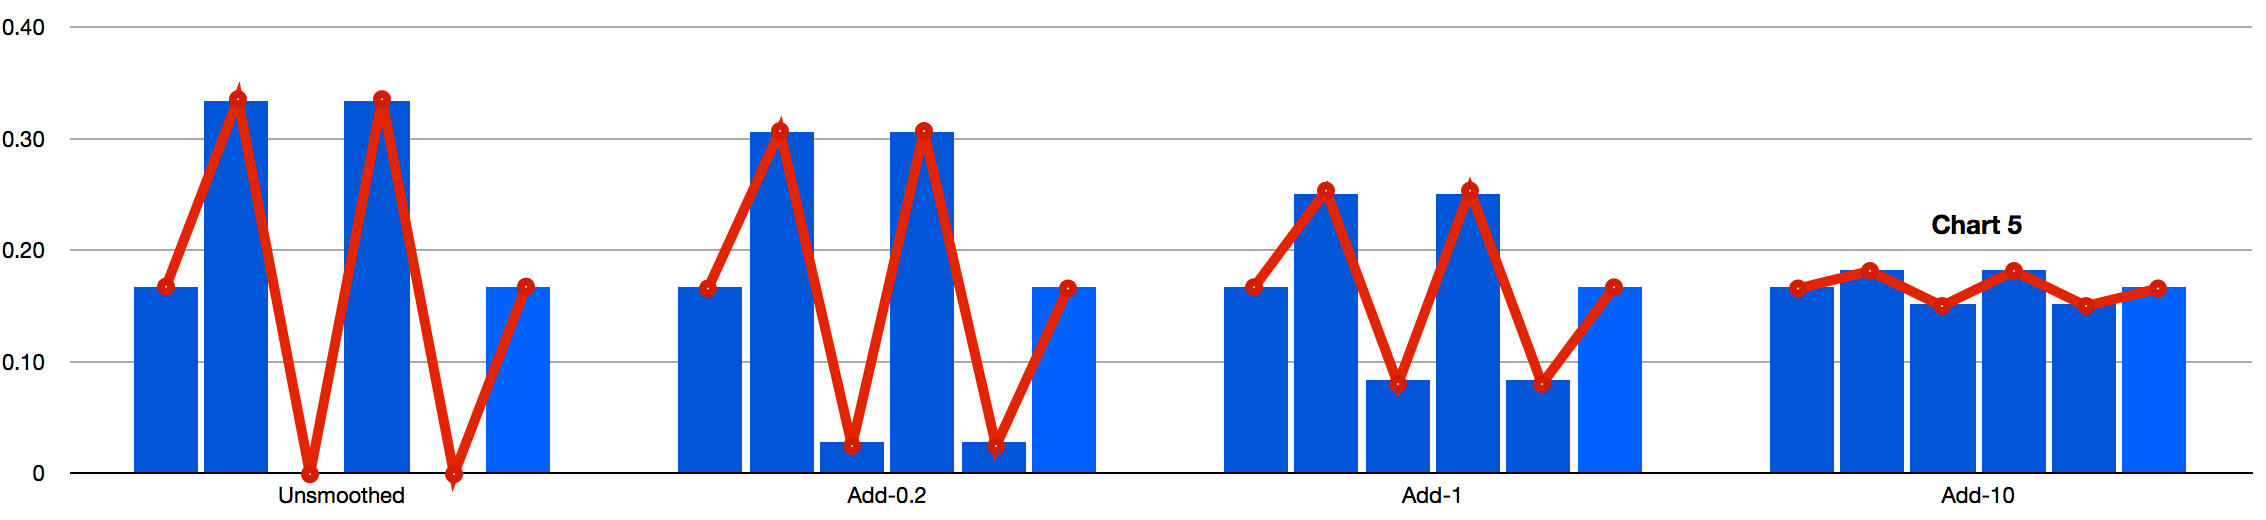
\includegraphics[width=0.9\textwidth]{smoothing.png}\end{center}

    \begin{itemize}
      \item (Partial) counts are ``stolen'' from high-count items and ``given'' to low-count items
      \item Extreme values are smoothed the most
      \item The impact of smoothing is depends on the relative values of $\lambda$ and the counts.
      \item If there are few overall counts, then a relatively large $\lambda$ will over-smooth, making all values approximately the same likelihood.
      \item If there are many overall counts, then a relatively small $\lambda$ will not make much impact.
      \item $\lambda=0$ means no smoothing
      \item $\lambda=\infty$ means uniform distributiom (all have equal probability)
    \end{itemize}

  \item Smoothing changes the relative probabilities of things most when there are low overall counts
    \begin{itemize}
      \item This is good because low counts means low evidence and, thus, low confidence
      \item We want the impact of evidence to be strong only when we have high confidence
      \item For na\"{i}ve Bayes, we always compare $p(F \mid L_1)$ to $p(F \mid L_2)$
      \item If counts $C(F,L_1)$ and $C(F,L_2)$ are small, we want smoothing to push the relative probabilities together, thus giving them a smaller impact in the NB calculation.  (The most extreme example is equal probabilities, which contribute no information to NB vs zero counts, which completely dominate the NB calculation).
      \item If counts $C(F,L_1)$ and $C(F,L_2)$ are large, we do not want smoothing to have a large impact on the relative probabilities
      \\
      \item For things with low counts (0 vs. 1), smoothing pushes the relative probabilities close together \\
        If $C(A)=1$, $C(B)=0$
        \begin{itemize}
          \item $p(A)=\frac{1}{1} = \mathbf{1.0}$ and 
                $p(B) = \mathbf{0.0}$
          \item $p_{+1}(A)=\frac{2}{3} = \mathbf{0.67}$ and 
                $p_{+1}(B) = \mathbf{0.33}$
        \end{itemize}

        If $C(A)=2$, $C(B)=1$
        \begin{itemize}
          \item $p(A)=\frac{2}{3} = \mathbf{0.67}$ and 
                $p(B) = \mathbf{0.33}$
          \item $p_{+1}(A)=\frac{3}{5} = \mathbf{0.60}$ and 
                $p_{+1}(B) = \mathbf{0.40}$
        \end{itemize}

      \item For things with non-trivial counts, the smoothed relative probabilities don't change much. 
        If $C(A)=30$, $C(B)=0$
        \begin{itemize}
          \item $p(A)=\frac{30}{30} = \mathbf{1.0}$ and 
                $p(B) = \mathbf{0.0}$
          \item $p_{+1}(A)=\frac{31}{32} = \mathbf{0.97}$ and 
                $p_{+1}(B) = \mathbf{0.03}$
        \end{itemize}

        If $C(A)=20$, $C(B)=10$
        \begin{itemize}
          \item $p(A)=\frac{20}{30} = \mathbf{0.67}$ and 
                $p(B) = \mathbf{0.33}$
          \item $p_{+1}(A)=\frac{21}{32} = \mathbf{0.66}$ and 
                $p_{+1}(B) = \mathbf{0.44}$
        \end{itemize}
    \end{itemize}
\end{itemize}


Classify \textit{Austria} with Add-1 smoothing

\begin{itemize}
  \item The prior
    \begin{itemize}
      \item We do \textit{not} need (or want) to smooth the prior distribution $p(Label)$
      \item Smoothing is useful when we have very low or zero counts
      \item Counts of labels will never be so low that we can't estimate them
    \end{itemize}

  \item Likelihood of the evidence
    \begin{itemize}
      \item $p(end=ia \mid label=location) = \frac{C(end=ia, label=location)+1}{C(label=location)+|end~values|} = \frac{4+1}{6+4} = \frac{5}{10} = 0.50$
      \item $p(end=ia \mid label=person) = \frac{C(end=ia, label=person)}{C(label=person)+|end~values|} = \frac{1+1}{4+4} = \frac{2}{8} = 0.25$
      \\
      \item $p(start=A \mid label=location) = \frac{C(start=A, label=location)}{C(label=location)+|start~values|} = \frac{0+1}{6+6} = \frac{1}{12} = 0.08$
      \item $p(start=A \mid label=person) = \frac{C(start=A, label=person)}{C(label=person)+|start~values|} = \frac{1+1}{4+6} = \frac{2}{10} = 0.20$
      \\
      \item No longer have zeros (this is essential)
      \item $start=A$ relative probabilities are pushed closer together than $end=ia$ since there is less evidence for either label

    \end{itemize}


  \item The posterior
    \begin{itemize}
      \item $p(label=location \mid start=A, end=ia) \\
            ~ = p(label=location) \cdot p(start=A \mid label=location) \cdot p(end=ia \mid label=location) \\
            ~ = 0.6 \cdot 0.08 \cdot 0.50 = \mathbf{0.024}$
      \item $p(label=person \mid start=A, end=ia) \\
            ~ = p(label=person) \cdot p(start=A \mid label=person) \cdot p(end=ia \mid label=person) \\
            ~ = 0.4 \cdot 0.20 \cdot 0.25 = \mathbf{0.020}$
    \end{itemize}
  \item Since $0.024 > 0.020$, we pick the label \textit{location}
  \item So smoothing fixed this classification example!
\end{itemize}




\section{Smoothing over unknowable things}

\begin{itemize}
  \item In the tennis example, we have four features, and all of their possible values are known.
  \item What happens if the set of possible values is unknown?
  \item What if we want to classify the word ``Zambia'' as a person or location?
    \begin{itemize}
      \item $p_{+1}(end=ia \mid location) = \frac{C(end=ia \mid location) + 1}{C(location) + |end~values|} = \frac{4+1}{6+4} = \frac{5}{10} = 0.50$
      \item $p_{+1}(end=ia \mid person) = \frac{C(end=ia \mid person) + 1}{C(person) + |end~values|} = \frac{1+1}{4+4} = \frac{2}{8} = 0.25$
      \\
      \item $p_{+1}(start=Z \mid location) = \frac{C(start=Z \mid location)}{C(location) + |start~values|} = \frac{0+1}{6+6} = \frac{1}{12} = 0.08$
      \item $p_{+1}(start=Z \mid person) = \frac{C(start=Z \mid person)}{C(person) + |start~values|} = \frac{0+1}{4+6} = \frac{1}{10} = 0.10$
    \end{itemize}
  \item So where does $start=Z$ fit in to the PD?
    \begin{itemize}
      \item $p_{+1}(start=B \mid location) = \frac{C(start=B \mid location)}{C(location) + |start~values|} = \frac{2+1}{6+6} = \frac{3}{12} = 0.25$
      \item $p_{+1}(start=M \mid location) = \frac{C(start=M \mid location)}{C(location) + |start~values|} = \frac{0+1}{6+6} = \frac{1}{12} = 0.08$
      \item $p_{+1}(start=L \mid location) = \frac{C(start=L \mid location)}{C(location) + |start~values|} = \frac{1+1}{6+6} = \frac{2}{12} = 0.17$
      \item $p_{+1}(start=N \mid location) = \frac{C(start=N \mid location)}{C(location) + |start~values|} = \frac{2+1}{6+6} = \frac{3}{12} = 0.25$
      \item $p_{+1}(start=E \mid location) = \frac{C(start=E \mid location)}{C(location) + |start~values|} = \frac{1+1}{6+6} = \frac{2}{12} = 0.17$
      \item $p_{+1}(start=A \mid location) = \frac{C(start=A \mid location)}{C(location) + |start~values|} = \frac{0+1}{6+6} = \frac{1}{12} = 0.08$
      \item $p_{+1}(start=Z \mid location) = \frac{C(start=Z \mid location)}{C(location) + |start~values|} = \frac{0+1}{6+6} = \frac{1}{12} = 0.08$

      \item But $(3+1+2+3+2+1+1)/12 = 13/12$!
      \item We had to add $|start~values|$ to the denominator to keep the PD valid, but we failed.
      \item We should have accounted for $Z$ by adding it to the set of start values
      \item So how many unseen start values are there?  $A$-$Z$?  Plus $a$-$z$?  Plus $A$-$\Omega$?
      \item Sometimes we don't know how many possible values there are.  Like when its all of the words.
      \item Add-$\lambda$ smoothing doesn't handle this nicely.
      \item Solution? Use the set of known values and hope for the best.
    \end{itemize}


\end{itemize}




\section{Features occurring more than once per instance}

\begin{itemize}
  \item Up to this point we have only worked with instances that have exactly one value of each feature per instance.
  \item But sometimes we want to classify data that has feaures that appear multiple times per instance, possibly with the same values.
  \item A canoncial example of this is when we are classifying text and we simply use the words in the text as features.

  \item The dataset:
\end{itemize}
    \begin{verbatim}
    the movie was great and the acting was great , so i loved it, positive
    i loved the movie dispite the terrible acting, positive
    the plot was great , but overall it was terrible, negative
    that movie was terrible, negative
    the movie had a terrible ending, but was great anyway, positive
    what a terrible movie, negative
    i've never seen anything so terrible, negative\end{verbatim}

\begin{itemize}
  \item Could have stopwords removed and be transformed to:
\end{itemize}
    \begin{verbatim}
    word=movie,word=great,word=acting,word=great,word=loved,5words=true,positive
    word=loved,word=movie,word=terrible,word=acting,5words=true,positive
    word=plot,word=great,word=terrible,5words=true,negative
    word=movie,word=terrible,5words=false,negative
    word=movie,word=terrible,word=ending,word=great,5words=true,positive
    word=terrible,word=movie,5words=false,negative
    word=terrible,5words=true,negative\end{verbatim}

\begin{itemize}
  \item 2 features: \textit{word} and \textit{5words}
\end{itemize}

Counting with duplicate features

\begin{itemize}
  \item If a feature can appear multiple times per instance, we have to count them all
  \item So the full counts are $C(feature=F,label=L)$.
  \item But we also need to make our probability calculation more precise
  \item Before, we said: $p(feature=F \mid label=L) = \frac{C(feature=F,label=L)}{C(label=L)}$
    \begin{itemize}
      \item This would mean, for our data:
      \item $p(word=great \mid label=positive) = \frac{C(word=great, label=positive)}{C(label=positive)} = \frac{3}{3} = 1.0$
      \item This would mean that if the instance is \textit{positive}, then it \textit{definitely} has ``great'' in it... which is false.
      \item Moreover, this would not make a valid probability distribution, since there are other words that also appear with \textit{positive}.
      \item The probability is wrong because we counted multiple \textit{word} features per instance, but only one \textit{label} feature per instance.
    \end{itemize}
  \item Since there is no longer one feature of each time per instance, we have to make our probability calculations more precise.
  \item $p(feature=F \mid label=L) = \frac{C(feature=F,label=L)}{\sum_f C(feature=f,label=L)}$
    \begin{itemize}
      \item So we are no longer dividing the number of instance with the label and feature by the number of instances with the label.
      \item Instead, we have to count the number of (label,value) pairs extracted from the data for the particular feature, including multiple identical pairs in the same instance
    \end{itemize}
  \item The probability $p(feature=F \mid label=L)$ is the proportion of times the particular feature was $F$ in an instance with label $L$ out of the total number of times the particular feature appeared in an instance with label $L$
  \item $p(word=great \mid label=positive) = \frac{C(word=great,label=positive)}{\sum_f C(word=f,label=positive)} = \frac{3}{13} = 0.23$ \\
  $p(word=great \mid label=negative) = \frac{C(word=great,label=negative)}{\sum_f C(word=f,label=negative)} = \frac{1}{8} = 0.13$
  \item Note that we still calculate the prior the same way: percentage of \textit{instances} that have the particular label.
\end{itemize}





\section{Evaluating}

\begin{itemize}
  \item How do we tell if our classifier works?
    \begin{itemize}
      \item Evaluating on the training data doesn't tell us about performance on new data
    \end{itemize}
  \item How do we set hyper-parameters (e.g. $\lambda$) without cheating?
    \begin{itemize}
      \item Tuning them to the test set wouldn't tell us about performance on new data
    \end{itemize}
\end{itemize}


Data Split

\begin{itemize}
  \item Divide labeled data into three groups: \textbf{train}, \textbf{development (dev)}, and \textbf{test}
  \item Use only the \textit{train} data to set parameters (take counts)
  \item Test against the \textit{dev} data using various choices for hyper-parameters (e.g. $\lambda$) to figure out the best settings.
  \item When all development is done, and you are ready to get final results for publication, evaluate \textit{just once} on the \textit{test} data, and record the results as your final results.
\end{itemize}


Data Size

\begin{itemize}
  \item Larger training set means that we will have better count estimates and, therefore, better model parameter estimates
  \item Larger dev and test sets mean that we can trust the results more
\end{itemize}


Accuracy

\begin{itemize}
  \item Proportion of test instances that are labeled correctly: $\frac{C(correct)}{C(total)}$
  \item 100 instances, 70 correctly labeled: 70\% correct
  \item Simple and intuitive, but can be misleading
  \item 100 instances, 80 are \textit{not spam}
    \begin{itemize}
      \item If the system just always outputs \textit{not spam}, then accuracy is 80\%
      \item But the model is worthless!
    \end{itemize}
\end{itemize}


Precision and Recall

\begin{itemize}
  \item Precision: Out of those that we labeled ``spam'', what proportion are actually spam? \\ 
        $p(is~spam \mid says~``spam")$
  \item Recall: Out of those that are actually spam, what proportion did we correctly label as ``spam''? \\ 
        $p(says~``spam" \mid is~``spam")$
  \item Categorize kinds of correctness and mistakes for \textit{spam} \\
        true positive (tp):  model says ``spam'',     actually spam     \\
        false positive (fp): model says ``spam'',     actually not spam \\
        false negative (fn): model says ``not spam'', actually spam     \\
        true negative (tn):  model says ``not spam'', actually not spam 
 
  \item $precision = \frac{tp}{tp + fp}$ ~~~~~~ $recall = \frac{tp}{tp + fn}$
  \item $F_1$-score: A way of combining precision and recall into one number (using the harmonic mean)
    \begin{itemize}
      \item $F_1 = 2 \cdot \frac{P \cdot R}{P + R}$
    \end{itemize}

  \item 100 instances:
    \begin{itemize}
      \item P \& R on \textit{spam} \\
        \begin{tabular}{|c|c|c|c|}
          \cline{3-4}
          \multicolumn{1}{ c }{} & \multicolumn{1}{ c| }{} & \multicolumn{2}{|c|}{model says} \\
          \cline{3-4}
          \multicolumn{1}{ c }{} & \multicolumn{1}{ c| }{} & spam & not spam \\
          \hline
          \multirow{2}{*}{truth} & spam     & TP = 20 & FN = 10 \\
          \cline{2-4}
                                 & not spam & FP = 15 & TN = 55 \\
          \hline
        \end{tabular} 
        \\
        \begin{itemize}
          \item Accuracy is 0.75
          \item Precision = $\frac{tp}{tp + fp} = \frac{20}{20 + 15} = 0.57$
          \item Recall =    $\frac{tp}{tp + fn} = \frac{20}{20 + 10} = 0.67$
          \item $F_1 = 2 \cdot \frac{P \cdot R}{P + R} = 2 \cdot \frac{0.57 \cdot 0.67}{0.57 + 0.67} = 0.62$
        \end{itemize} ~

      \item P \& R on \textit{not spam} \\
        \begin{tabular}{|c|c|c|c|}
          \cline{3-4}
          \multicolumn{1}{ c }{} & \multicolumn{1}{ c| }{} & \multicolumn{2}{|c|}{model says} \\
          \cline{3-4}
          \multicolumn{1}{ c }{} & \multicolumn{1}{ c| }{} & spam & not spam \\
          \hline
          \multirow{2}{*}{truth} & spam     & TN = 20 & FP = 10 \\
          \cline{2-4}
                                 & not spam & FN = 15 & TP = 55 \\
          \hline
        \end{tabular} 
        \\
        \begin{itemize}
          \item Accuracy is 0.75
          \item Precision = $\frac{tp}{tp + fp} = \frac{55}{55 + 10} = 0.85$
          \item Recall =    $\frac{tp}{tp + fn} = \frac{55}{55 + 15} = 0.79$
          \item $F_1 = 2 \cdot \frac{P \cdot R}{P + R} = 2 \cdot \frac{0.85 \cdot 0.79}{0.85 + 0.79} = 0.89$
        \end{itemize}
    \end{itemize}

  \item 100 instances, 80 are \textit{not spam}, and the system just always outputs \textit{not spam} 
    \begin{itemize}
      \item P \& R on \textit{spam} \\
        \begin{tabular}{|c|c|c|c|}
          \cline{3-4}
          \multicolumn{1}{ c }{} & \multicolumn{1}{ c| }{} & \multicolumn{2}{|c|}{model says} \\
          \cline{3-4}
          \multicolumn{1}{ c }{} & \multicolumn{1}{ c| }{} & spam & not spam \\
          \hline
          \multirow{2}{*}{truth} & spam     & TP = 0 & FN = 20 \\
          \cline{2-4}
                                 & not spam & FP = 0 & TN = 80 \\
          \hline
        \end{tabular} 
        \\
        \begin{itemize}
          \item Accuracy is 0.80
          \item Precision = $\frac{tp}{tp + fp} = \frac{0}{0 +  0} = $ \textit{NaN}
          \item Recall =    $\frac{tp}{tp + fn} = \frac{0}{0 + 20} = 0.0$
          \item $F_1 = 2 \cdot \frac{P \cdot R}{P + R} =$ ?
        \end{itemize} ~

      \item P \& R on \textit{not spam} \\
        \begin{tabular}{|c|c|c|c|}
          \cline{3-4}
          \multicolumn{1}{ c }{} & \multicolumn{1}{ c| }{} & \multicolumn{2}{|c|}{model says} \\
          \cline{3-4}
          \multicolumn{1}{ c }{} & \multicolumn{1}{ c| }{} & spam & not spam \\
          \hline
          \multirow{2}{*}{truth} & spam     & TN = 0 & FP = 20 \\
          \cline{2-4}
                                 & not spam & FN = 0 & TP = 80 \\
          \hline
        \end{tabular} 
        \\
        \begin{itemize}
          \item Accuracy is 0.80
          \item Precision = $\frac{tp}{tp + fp} = \frac{80}{80 + 20} = 0.80$
          \item Recall =    $\frac{tp}{tp + fn} = \frac{80}{80 +  0} = 1.00$
          \item $F_1 = 2 \cdot \frac{P \cdot R}{P + R} = 2 \cdot \frac{0.80 \cdot 1.00}{0.80 + 1.00} = 0.89$
        \end{itemize}
    \end{itemize}
\end{itemize}








\section{Semi-Supervised Learning for Na\"{i}ve Bayes}

\begin{itemize}
  \item At this point, we know how to train a na\"{i}ve Bayes classifier from fully-supervised data (every training instance has a label)
  \item Can we use (lots of) unlabeled data to improve a NB classifier trained on just a small amount of labeled data?
  \item Can we learn a NB classifier with out any labeled data?
\end{itemize}

An excellent tutorial that carefully explains everything necessary to implement Gibbs sampling for na\"{i}ve Bayes:

\begin{itemize}
  \item Philip Resnik and Eric Hardisty.  ``Gibbs Sampling for the Uninitiated''.  June 2010.\\  \url{http://www.cs.umd.edu/~hardisty/papers/gsfu.pdf}
\end{itemize}


Partial Supervision: The Idea

\begin{itemize}
  \item We know how to use NB to classify if we have labeled data
  \item If we have unlabeled data, we can assign labels to all the instances, then it because labeled data, and we can use it for NB
  \item We don't want to just assign labels and assume that they are correct
  \item So we will make initial guesses for those labels, and iteratively revise them
  \item Critically, we won't revise by simply picking the most likely label.  We will choose probabilistically, based on the relatively probaiblities of the different labels.
\end{itemize}


The Algorithm

\begin{itemize}
  \item[1.] Make a NB classifier from any labeled data available.
  \item[2.] For each unlabeled instance:
    \begin{itemize}
      \item[a.] Use this classifier to calculate the probabilities of each label.
      \item[b.] Make a probabilty distribution out of all label probabilties (normalize them so that they add up to 1.0)
      \item[c.] Sample from the probability distribution by choosing a label with likelihood according to its probability
      \item[d.] Assign that chosen label as the label for the instance
    \end{itemize}
  \item[3.] For some large number of iterations, for each unlabeled instance:
    \begin{itemize}
      \item[a.] Make a NB classifier from all the instances and their current labels.
      \item[c.] Use this classifier to calculate the probabilities of each label.
      \item[c.] Make a probabilty distribution out of all label probabilties (normalize them so that they add up to 1.0)
      \item[d.] Sample from the probability distribution by choosing a label with likelihood according to its probability
      \item[e.] Assign that chosen label as the revised label for the instance
      \item[f.] Copy the instance with its new label into a ``repository'' of labeled instances.
    \end{itemize}
  \item[4.] Make a final NB classifier from all of the labeled instances in the ``repository'' that we built up while we were sampling.
  \item We don't revise the labels of the supervised instances because we assume that they are correct (unless we don't trust them, or think they are out-of-date).
  \item Always making probabilistic label choices prevents us from just accepting the MLE and getting stuck.
  \item The choices will allow us to ``walk'' around the space of labels, where most of the walking happens in area that lead to better parameters.
\end{itemize}


Why does this work?

\begin{itemize}
  \item Basically, it learns how group associated feature values together, and how to push different labels apart.
  \item We start with a ``best guess'' based on information we have, and revise our guesses over time.
  \item We don't just walk ``uphill'' based on the MLE.  
  \item Instead we allow ourselves to explore lots of label choices, some of which may be very different from the MLE.
  \item As we become more confident in a judgement, its label is less likely to change because more of the similar instances will be using that label, which gives it a high probability.
\end{itemize}

Markov Chain Monte Carlo

\begin{itemize}
  \item Markov: Uses the ``Markov principle'' which says to make decisions based only on recent information
    \begin{itemize}
      \item We use only the current set of labels, not the full history of labels.
    \end{itemize}
  \item Chain: Start with an initial set of labels, use it to change one label, then move to the next label and change it based on the new set of labels.  Repeat for a long time.
  \item Monte Carlo: Each step in the chain has chance involved
    \begin{itemize}
      \item We choose the next label by chance according to the relative probabilities of the labels.
      \item Named for Monte Carlo in Monaco and the Monte Carlo Casino
    \end{itemize}
\end{itemize}



\section{Clustering}

\begin{itemize}
  \item Until now, all our classifiers have been learned from fully-supervised data (every training instance has a label)
  \item Can we learn a classifier when we have no labels at all?
  \item \textbf{Clustering} is when we try to automatically induce groupings without labels.
\end{itemize}

K-Means

\begin{itemize}
  \item[1.] Plot all instances in space
  \item[2.] Choose $K$ of them to be initial centroids
  \item[3.] For each instance, associate it with its nearest centroid
  \item[4.] Update each centroid to the centroid of its currently-assocated instances
  \item[5.] Repeat step 3-4 until the centroids stop moving
  \item[6.] For new instances, classify based on their nearest centroid
\end{itemize}


\end{document}

